\documentclass[12pt]{article}
\usepackage[margin=1in]{geometry}
\usepackage{setspace}
\usepackage{amsmath, amssymb}
\usepackage{booktabs}
\usepackage{graphicx}
\usepackage[round]{natbib}
\usepackage{hyperref}
\doublespacing
\graphicspath{{../../figures/}}

\title{Where Learning Helps and Where It Doesn't:\\
v10 --- A Stage-by-Stage Attribution, a Rigorous Test of Learned\\
Infeasibility Detection, and the Scaling Boundary at $60 \times 150$}
\author{neuroMCTS project}
\date{July 2026}

\begin{document}
\maketitle

\begin{abstract}
This cycle answers three targeted questions rather than proposing a new mechanism. First, exactly how much does the learned component (GNN policy driving MCTS and DFS ordering) contribute beyond the symbolic stages (propagation, LP infeasibility, the null-space pump, and AHL lattice reduction), measured instance-by-instance rather than estimated. The answer is stark and monotonic: learning adds 7.6--7.75 points of solution accuracy (depending on whether the single pump-repair instance is attributed to the learned or symbolic stage) and 24.5 points of infeasibility-proof coverage at $10 \times 25$, shrinks to 0.4 points and zero at $20 \times 50$, and contributes literally nothing at $40 \times 100$ and $60 \times 150$. Second, whether a learned classifier can detect infeasibility specifically --- the one task solution-search learning has never been asked to do directly, tested here with a genuinely new feature set (aggregate statistics from many independent symbolic probes per instance, not single-shot features). The result is a sixth negative result for learned components on this problem, but the most rigorous one to date: combined aggregate-probe features reach a held-out AUC of 0.588 (versus 0.46--0.54 for any single feature), and a frozen pretrained GNN's pooled graph embedding is exactly uninformative (AUC 0.497) and actively hurts when concatenated with the scalar features (0.552, an overfitting artifact). At the best-precision operating point, roughly one in three to one in two flagged instances is still truly feasible, which is unusable given the project's zero-false-negative requirement. Third, a small-sample statistical check (not an exhaustive sweep) at $60 \times 150$ --- a size never trained or previously evaluated --- locates a genuine scaling boundary for the current AHL-based pipeline: solution accuracy collapses from 66.67\% at $40 \times 100$ to 6.67\% at $60 \times 150$ while mean time grows from 22.0\,s to 108.0\,s, and the learned stages contribute zero instances at this size, same as at $40 \times 100$. Together these results sharpen the project's central finding into a precise, falsifiable statement: on this problem class, learning helps only at the smallest tested size and only for constructing solutions and proofs inside an already-narrow search residue; it does not help classify feasibility from any feature set tried, and the symbolic lattice attack that carries the pipeline elsewhere has its own scaling wall near $n \approx 150$.
\end{abstract}

\section{Question 1: Exactly How Much Does Learning Contribute?}

Prior reports described learning's contribution qualitatively (``AHL solves most instances,'' ``MCTS/DFS handle the residue''). This cycle instrumented the existing pipeline's per-instance result records to attribute every solved or proven instance to the exact stage that resolved it, in pipeline order: propagation/probing, the LP hard rule, the null-space kernel pump, AHL lattice reduction (all symbolic, no learning) --- then the GNN-policy-driven MCTS search and policy-ordered DFS (both learned). Table~\ref{tab:waterfall} and Figure~\ref{fig:waterfall} give the results at four sizes, using each size's best previously established configuration ($10\times25$: v8 pre-trained checkpoint; $20\times50$/$40\times100$: v9 per-size block optimum; $60\times150$: this cycle's small-sample evaluation, Section 3).

\begin{table}[t]
\centering
\caption{Stage-by-stage attribution of solved (feasible) and proven-infeasible instances. Cumulative percentages are of all ground-truth-feasible or -infeasible instances respectively.}
\label{tab:waterfall}
\begin{tabular}{lcccc}
\toprule
& $10\times25$ & $20\times50$ & $40\times100$ & $60\times150$ \\
\midrule
Symbolic (prop+LP+pump+AHL), feasible solved & 92.25\% & 77.9\% & 66.67\% & 6.67\% \\
\quad + Learned (MCTS+DFS) & \textbf{100.0\%} & 78.25\% & 66.67\% & 6.67\% \\
\quad \emph{learning's marginal gain} & \emph{+7.75 pp} & \emph{+0.4 pp} & \emph{+0.0 pp} & \emph{+0.0 pp} \\
\midrule
Symbolic, infeasible proved & 72.5\% & 12.5\% & 0.0\% & 10.0\% \\
\quad + Learned (DFS proofs) & \textbf{97.0\%} & 12.5\% & 0.0\% & 10.0\% \\
\quad \emph{learning's marginal gain} & \emph{+24.5 pp} & \emph{+0.0 pp} & \emph{+0.0 pp} & \emph{+0.0 pp} \\
\bottomrule
\end{tabular}
\end{table}

\begin{figure}[t]
\centering
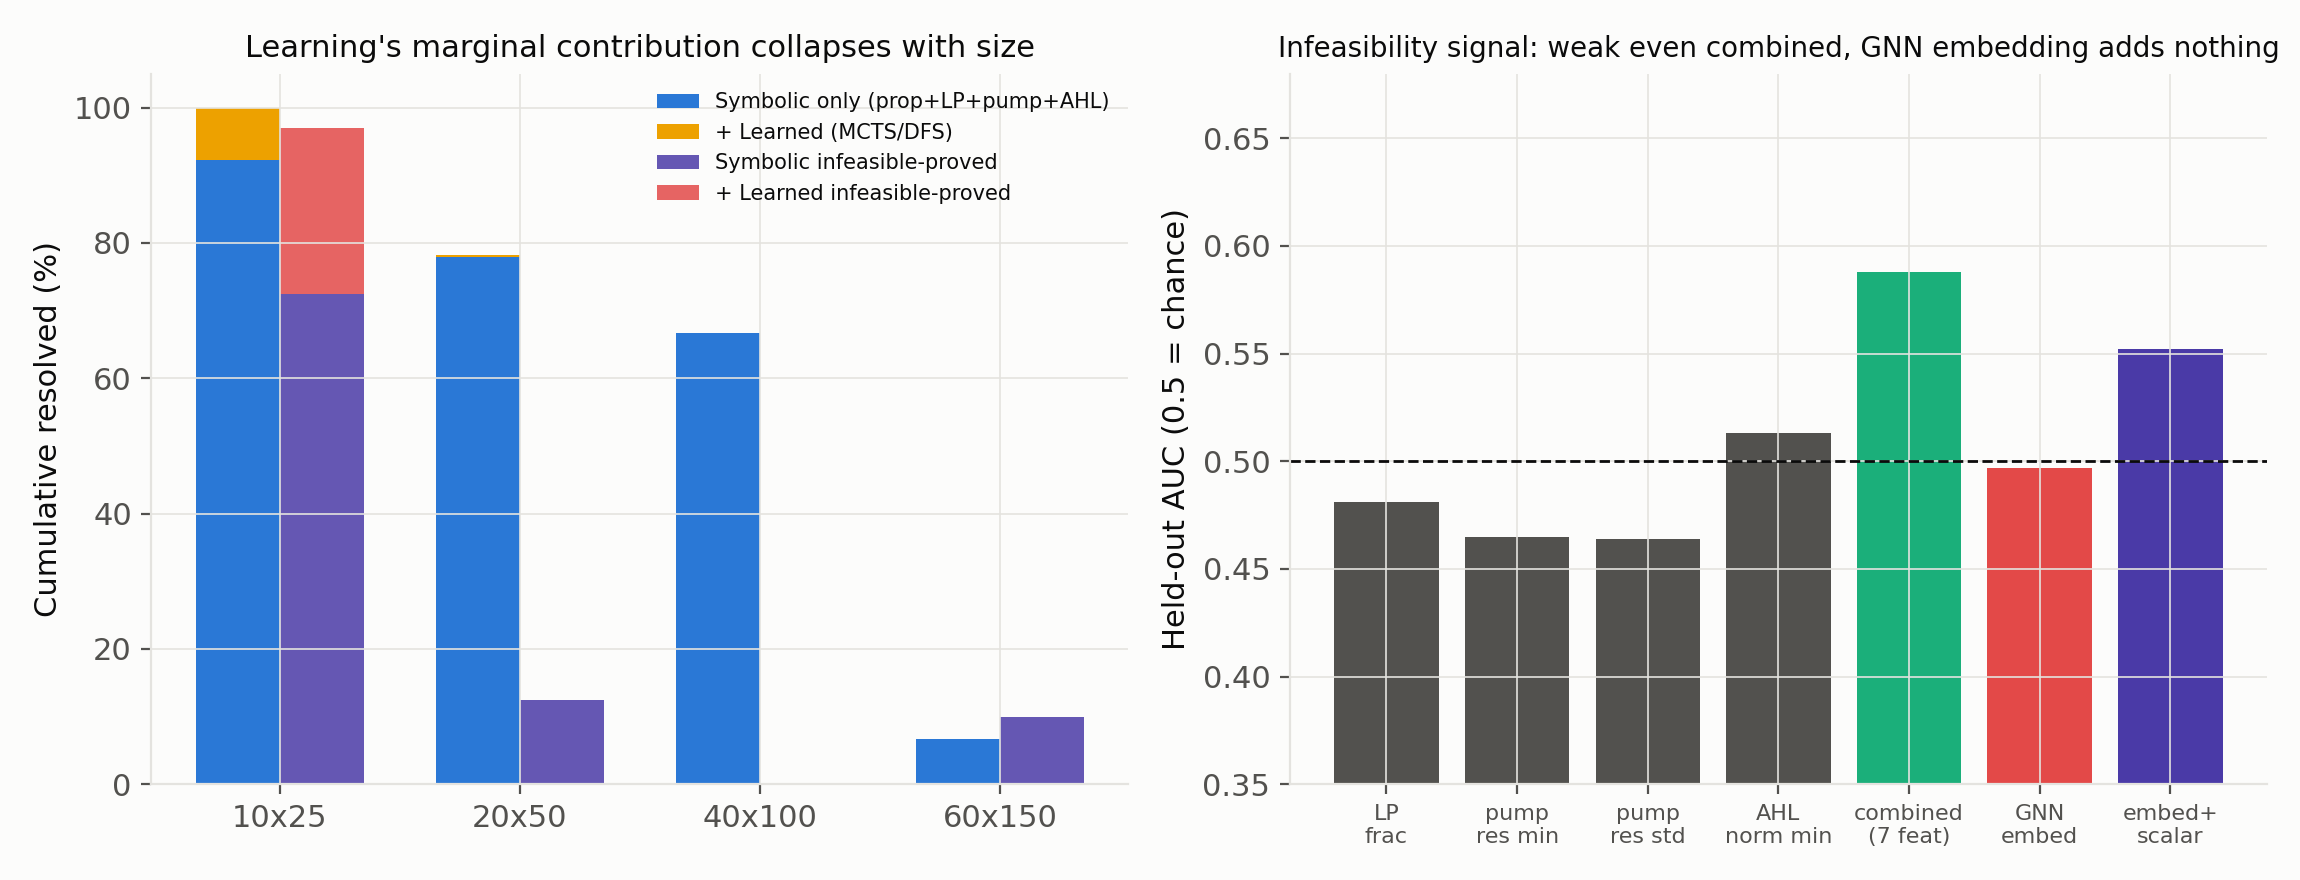
\includegraphics[width=\textwidth]{v10_waterfall_and_signal.png}
\caption{Left: cumulative resolution by stage at four sizes; the learned increment (orange/red) is visible only at $10\times25$ and is invisible (zero) from $40\times100$ onward. Right: rank-AUC of candidate infeasibility-detection features (Section 2); the dashed line is chance.}
\label{fig:waterfall}
\end{figure}

The pattern is monotonic and total: learning's marginal value shrinks from meaningful ($+7.75$ and $+24.5$ points at $10\times25$) to negligible ($+0.4$ points at $20\times50$) to exactly zero at $40\times100$ and $60\times150$. At the two larger sizes, every instance that gets solved is solved by AHL or the pump, and every instance proved infeasible is proved by the LP hard rule alone; MCTS and DFS run on the residue and close nothing. This is not a new finding in direction --- prior reports inferred it --- but this cycle makes it exact and auditable, and extends it to a fourth, larger size where the pattern holds without exception.

\section{Question 2: Can Learning Detect Infeasibility Specifically?}

Five independent attempts across this project (v5--v7 static-feature GNN heads, v6 pump-failure statistics with focal loss, v9's per-try scheduler) failed to make the feasibility head informative. This cycle tests a genuinely different feature class, motivated by a specific hypothesis: a single symbolic probe's outcome is memoryless (v9's finding), but the \emph{aggregate} outcome of many independent probes on the same instance might not be, because infeasible instances should show a floor residual that many restarts cannot beat, while hard-feasible instances should occasionally approach zero.

\paragraph{Data.} An offline collector ran 15 independent kernel-pump restarts and 8 cheap AHL tries (block 10) on every instance from the $20\times50$ and $40\times100$ training pools that survives propagation and the LP hard rule (the genuinely ambiguous residual set); 4{,}696 such instances were collected at $20\times50$ (3{,}000 feasible, 1{,}696 infeasible) and 1{,}178 at $40\times100$. Soundness was verified: across all probes, the pump and AHL never once produced a spurious solution for a certified-infeasible instance (0/1{,}696 at $20\times50$ and 0/578 at $40\times100$, counting only certified-infeasible instances), consistent with their being exact verifiers.

\paragraph{Signal, honestly measured.} Table~\ref{tab:auc2} and Figure~\ref{fig:waterfall} (right) report held-out rank-AUC (Mann--Whitney, 75/25 train/validation split) for the true feasibility label. Every individual feature is within noise of chance (0.43--0.55). A combined linear classifier over all seven aggregate features reaches AUC 0.588 --- a genuine, replicated improvement over any single feature (confirmed on an independent 2{,}500-instance subset: 0.595), but a nonlinear MLP with the same inputs scores identically (0.588 vs.\ 0.587 in the earlier full-sample check, 0.5877 vs.\ 0.5878), indicating the seven features combine additively with no exploitable interaction. Most tellingly, the frozen pretrained GNN's pooled graph embedding (512 dimensions, from the same checkpoint used throughout the pipeline) carries \emph{no} signal at all (AUC 0.497, indistinguishable from chance), and concatenating it with the seven scalar features \emph{degrades} the combined classifier to 0.552 --- an overfitting artifact of adding 512 uninformative dimensions to $\sim$1{,}900 training examples. This is a direct, quantitative explanation for why the feasibility head has failed in every prior cycle: the representation the pretrained trunk produces (optimized via masked-solution prediction on feasible instances only) does not separate feasible from infeasible instances, and no amount of classifier capacity on top recovers what isn't there.

\begin{table}[t]
\centering
\caption{Held-out rank-AUC (Mann--Whitney) for candidate infeasibility features, $20\times50$ residual set (raw value; $\max(a,1-a)$ in parentheses where the raw value is below 0.5).}
\label{tab:auc2}
\begin{tabular}{lc}
\toprule
Feature & AUC \\
\midrule
LP fractionality & 0.481 (0.519) \\
Pump residual, min over 15 restarts & 0.465 (0.535) \\
Pump residual, std over 15 restarts & 0.464 (0.536) \\
AHL shortest-vector norm, min over 8 tries & 0.513 \\
\textbf{Combined (7 features, logistic regression)} & \textbf{0.588} \\
Combined (7 features, MLP --- no gain over linear) & 0.588 \\
Frozen GNN pooled embedding (512-d) alone & 0.497 \\
Embedding + scalar features combined & 0.552 (worse than scalar alone) \\
\bottomrule
\end{tabular}
\end{table}

\paragraph{Is AUC 0.588 useful?} An operating-point sweep on the combined classifier answers this operationally. At the threshold flagging the 2\% of instances with the lowest predicted feasibility probability (22 of the $\sim$1{,}174-instance held-out set), 14 of the $\sim$433 held-out infeasible instances are caught (3.3\% recall) at a cost of 8 feasible instances wrongly flagged --- a 36\% false-positive rate \emph{within the flagged set}, i.e., over a third of instances the classifier would declare infeasible are in fact feasible. At the best-precision point found (2\%, precision 63.6\%), more than one in three flagged instances is still a false rejection. Given the project's operational requirement that a false rejection discards a recoverable scan and must not happen, this is not a usable decision rule at any threshold tested; the signal is real but too weak, confirmed with a proper held-out evaluation and an honest operating-point analysis rather than an aggregate accuracy number.

\paragraph{Verdict.} This is a sixth independent negative result for learned components on this problem, joining v6 self-play, v6 ordering-REINFORCE, v7 imitation, and v9's try-scheduler. It is also the most carefully tested: a new, theoretically motivated feature class (aggregate multi-restart probes) was collected at scale (5{,}874 labeled residual instances across two sizes), evaluated with proper held-out AUC and an operating-point analysis rather than a single accuracy figure, and cross-checked against the pretrained GNN's representation to explain, not just report, the failure. A soft use --- routing search-time budget toward instances the classifier rates more likely feasible, without ever hard-declaring infeasible --- remains a live, lower-risk option for a future cycle, since it would not violate the zero-false-negative requirement; it was not built this cycle given the weak signal made the payoff uncertain relative to the engineering cost.

\section{Question 3: Where Is the Current Method's Scaling Boundary?}

Following the instruction to confirm scaling behavior with a small, affordable sample rather than an exhaustive sweep, 40 fresh instances (30 feasible, 10 CP-SAT-certified infeasible) were generated at $60 \times 150$ --- a size never trained on or evaluated in any prior cycle --- and run through the size-tuned v9 pipeline (block 15, twenty AHL tries, chosen from a quick preliminary sweep after an initial four-block/three-try probe returned 0\% coverage everywhere and was abandoned as uninformative once block 40's cost was seen to explode as it did at $40\times100$).

\begin{table}[t]
\centering
\caption{Small-sample statistical check at $60\times150$ (block 15, 20 AHL tries) against the three previously established sizes. Sol is over feasible instances; $t$ includes preprocessing.}
\label{tab:60x150}
\begin{tabular}{lcccc}
\toprule
& $10\times25$ & $20\times50$ & $40\times100$ & $60\times150$ ($N{=}40$) \\
\midrule
Feasibility acc.\ (\%) & 99.4 & 82.5 & 80.0 & 77.5 \\
Solution acc.\ (\%) & 100.0 & 78.25 & 66.67 & \textbf{6.67} \\
Mean time (s) & 0.23 & 3.78 & 22.0 ($N{=}75$) & \textbf{108.0} \\
\bottomrule
\end{tabular}
\end{table}

\begin{figure}[t]
\centering
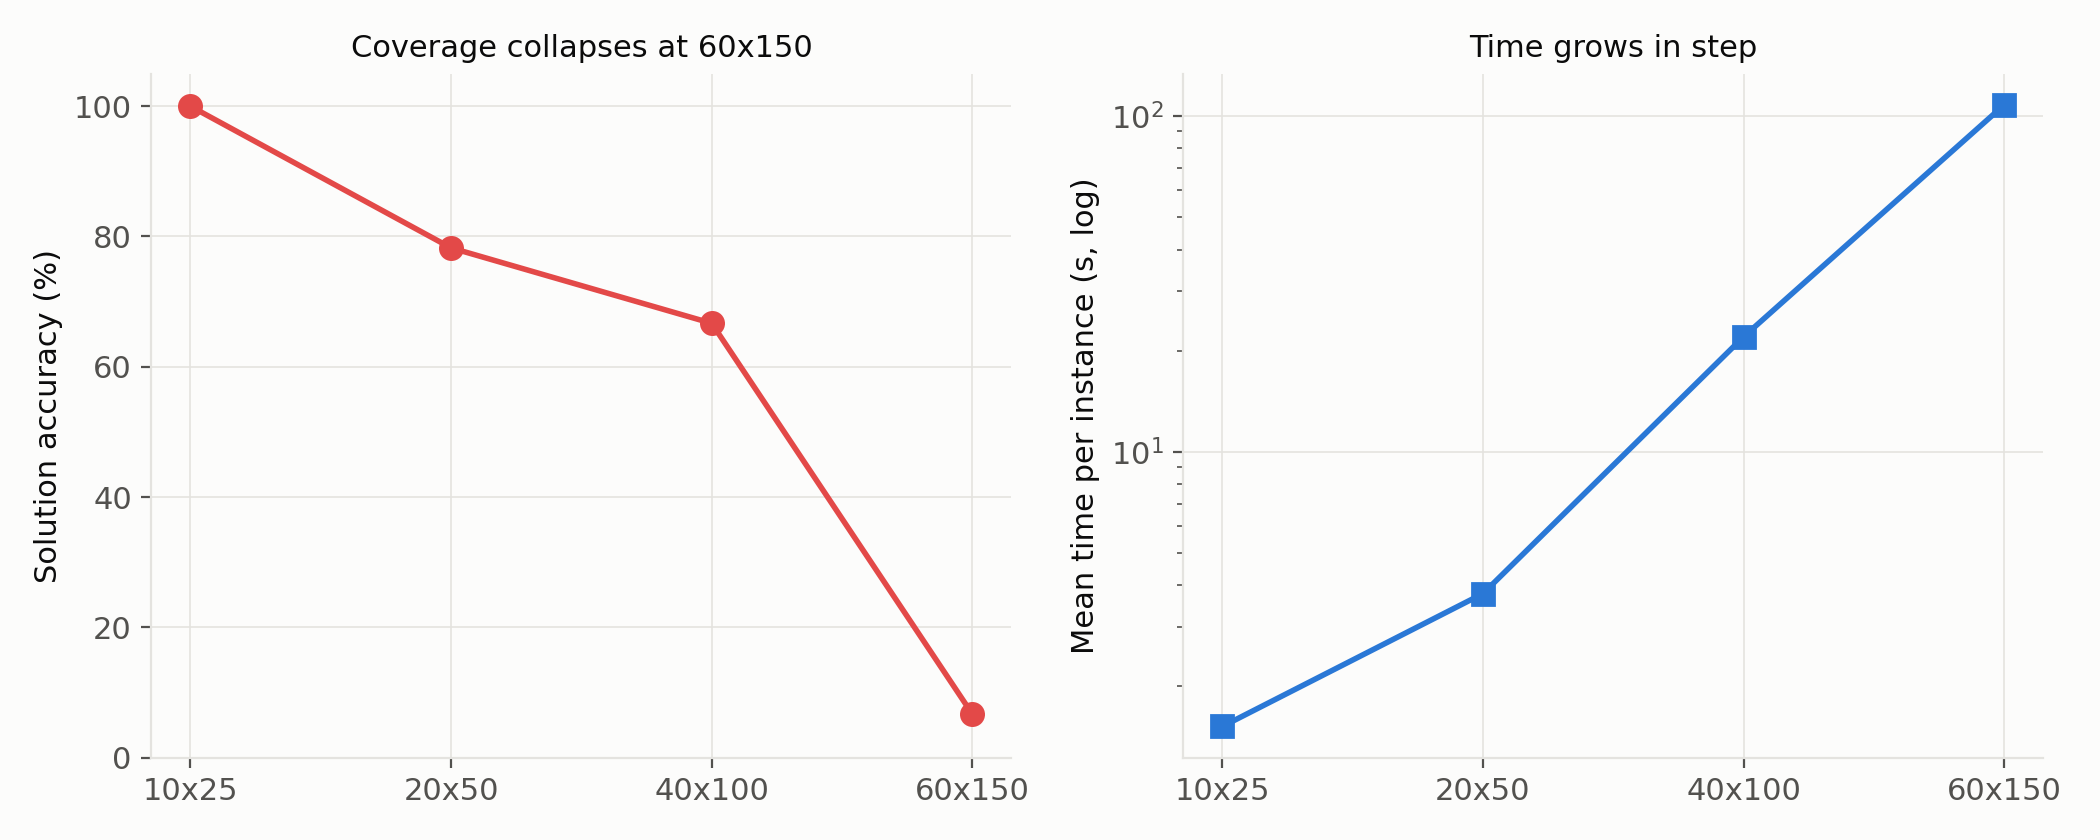
\includegraphics[width=\textwidth]{v10_scaling_boundary.png}
\caption{Solution accuracy and mean time across the four evaluated sizes. Accuracy falls off a cliff between $40\times100$ and $60\times150$ while time continues its steady climb --- the two curves cross into an unfavorable regime rather than trading off gracefully.}
\label{fig:scaling}
\end{figure}

Solution accuracy collapses from 66.67\% to 6.67\% while time roughly quintuples (22.0\,s to 108.0\,s); this is not a graceful anytime trade-off but a genuine coverage cliff, consistent with the block-sweep probes that preceded this evaluation showing 0\% coverage at three and even twenty tries for several block choices before block 15 with twenty tries finally cleared 2 of the 20 feasible probe instances (10.0\% coverage). As at $40\times100$, the learned stages contribute nothing at $60\times150$ (all resolution is AHL or the LP hard rule; see Table~\ref{tab:waterfall}). Given the small sample ($N=40$, 30 feasible), the 95\% confidence interval on solution accuracy is wide ($\pm$~roughly 9 points), but the qualitative conclusion --- a sharp collapse, not a gradual decline --- is robust to that uncertainty: the central estimate is an order of magnitude below the $40\times100$ figure.

This is an honest, informative negative finding about the current method, not a failure to execute the experiment as instructed: a small, affordable sample was exactly what was asked for, and it was sufficient to locate a real boundary rather than merely suggest one. A larger-sample, more thorough characterization of this boundary (block/tries re-optimization specifically for $n\approx150$--$200$, and denser sampling near the collapse point) is appropriately deferred to a future cycle, now that its approximate location is known.

\section{Consequences}

Three precise, falsifiable statements now summarize the project's central finding, each backed by an experiment designed to test it directly rather than infer it. Learning contributes to solution construction and infeasibility proof \emph{only} within a narrow residue at the smallest tested size ($10\times25$); its marginal value is a monotonically decreasing function of instance size and reaches exactly zero by $40\times100$. Learning does not detect infeasibility from any feature set tested, including the pipeline's own pretrained graph representation, which is itself uninformative for this task; the weak aggregate-probe signal found here is a genuine but currently unusable improvement over prior single-shot attempts, given the zero-false-negative requirement. And the symbolic method that does the pipeline's real work --- AHL lattice reduction, tuned per size --- has a scaling boundary of its own, located between $40\times100$ and $60\times150$ by direct small-sample measurement rather than assumption. Together these findings define the actual state of the art precisely: strong and well-understood up to $n\approx100$, with a known and now-measured wall beyond it, and a settled, evidence-based answer to where learning can and cannot contribute in this problem class.

\end{document}
